x\chapter{光の状態
}

コヒーレント状態$|\alpha\rangle$は、理想的なレーザー光を表している量子状態で、複素振幅$\alpha=x+iy$を持っている。また複素平面上で平均ベクトル$(x,y)^T$と共分散行列
$$
\begin{pmatrix}
1/4&0\\
0&1/4
\end{pmatrix}
$$
の正規分布に従って揺らいでいる。そしてコヒーレント状態を一般化したものが量子ガウス状態である。量子ガウス状態は、平均ベクトル$(x,y)^T$と共分散行列
$$
\begin{pmatrix}
a&c\\
c&b
\end{pmatrix}
$$
で表される。ただし共分散行列の要素は、関係式
$a+b\geq 0$,$ab-c^2\geq1/16$
を満たす必要がある。
スクイズド状態$|\alpha,\zeta\rangle$はガウス状態の一種で、図1のように量子揺らぎを持っている。スクイズド状態は、複素数$\alpha,\zeta$によって特徴づけられる。特に$\alpha$を$x+iy$,$\zeta$を$re^{i\theta}$とすると、
\begin{equation}
\begin{split}
a&=1/4[\cosh 2r-\sinh 2r\cos\theta]\\
b&=1/4[\cosh 2r+\sinh 2r\cos\theta]\\
c&=1/4\sinh 2r\sin\theta
\end{split}
\end{equation}
によって平均ベクトル$(x,y)^T$と共分散行列
\begin{equation}
\begin{pmatrix}
a&c\\
c&b
\end{pmatrix}
\end{equation}
が決まる。

\begin{figure}[htbp]
        \centering   
        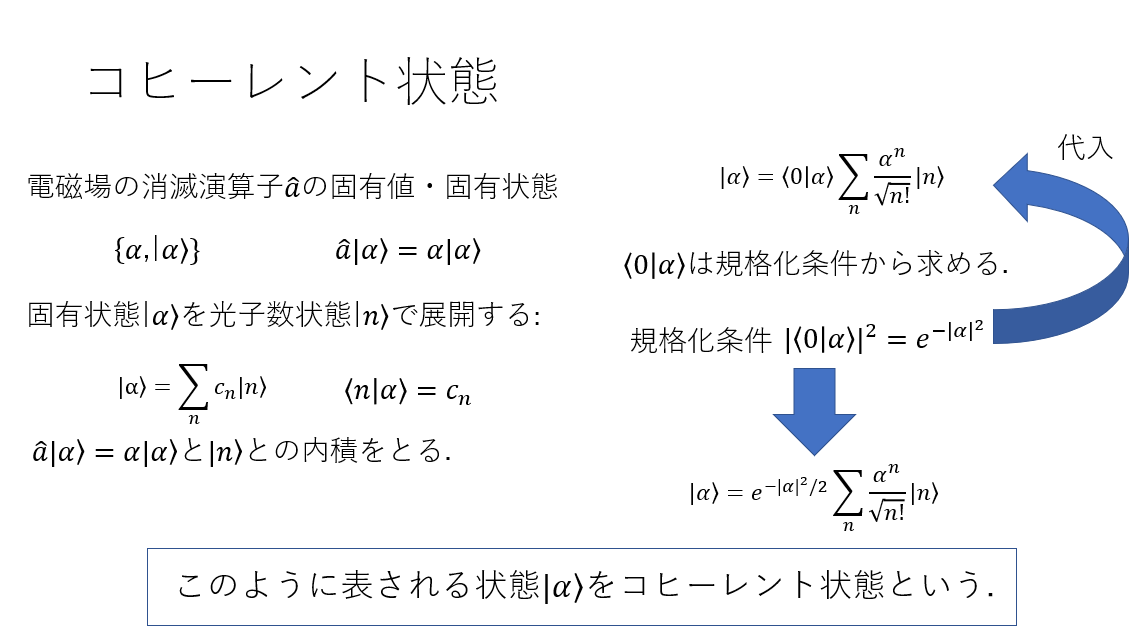
\includegraphics[width=1.0\textwidth]{img/zemi9.png}
        \caption[sample image (png)]{コヒーレント状態.}
        \label{Fig:1_5_1}
    \end{figure}
    
    \figref{Fig:1_5_1}はコヒーレント状態の定義を表している。コヒーレント状態は電磁場の消滅演算子の固有状態として与えられる。
    
\begin{figure}[htbp]
        \centering   
        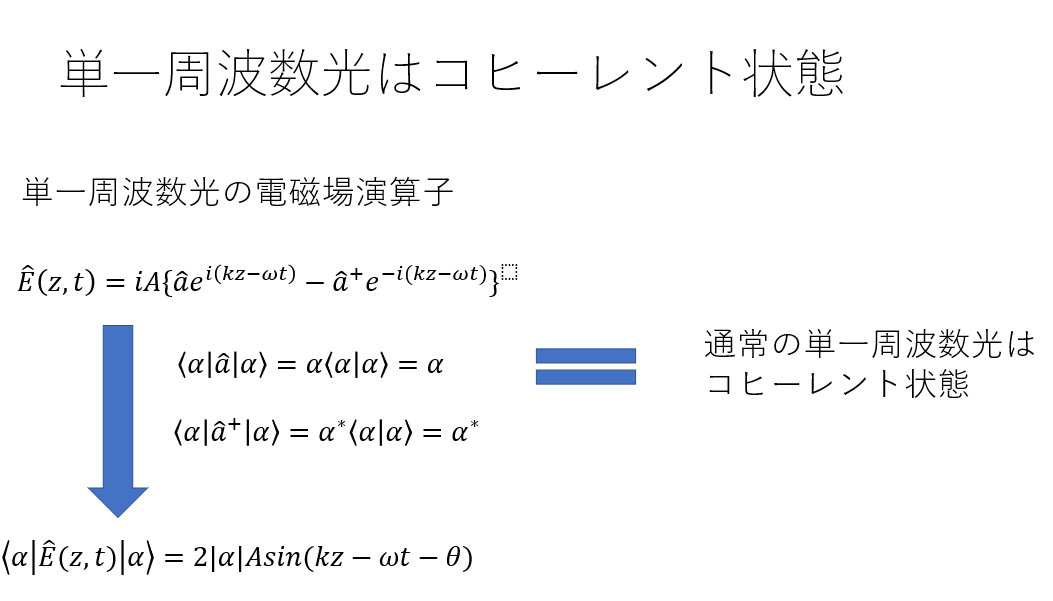
\includegraphics[width=1.0\textwidth]{img/zemi10.png}
        \caption[sample image (png)]{単一周波数光はコヒーレント状態.}
        \label{Fig:1_5_2}
    \end{figure}
    
    \figref{Fig:1_5_2}に示すように通常の単一周波数光はコヒーレント状態としてあらわされる。

\begin{figure}[htbp]
        \centering   
        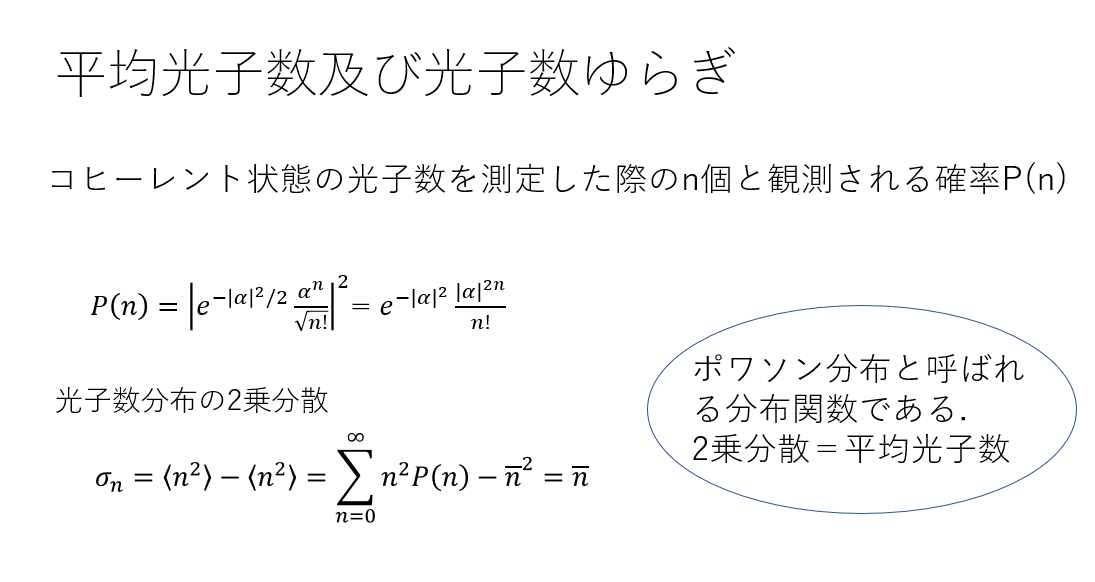
\includegraphics[width=1.0\textwidth]{img/zemi11.png}
        \caption[sample image (png)]{平均光子数及び光子数ゆらぎ.}
        \label{Fig:1_5_3}
    \end{figure}
    
    \figref{Fig:1_5_3}はコヒーレント状態の光子数を測定した際の$n$個と観測される確率$P(n)$について説明している。$P(n)$はポワソン分布と呼ばれる分布関数である。

\begin{figure}[htbp]
        \centering   
        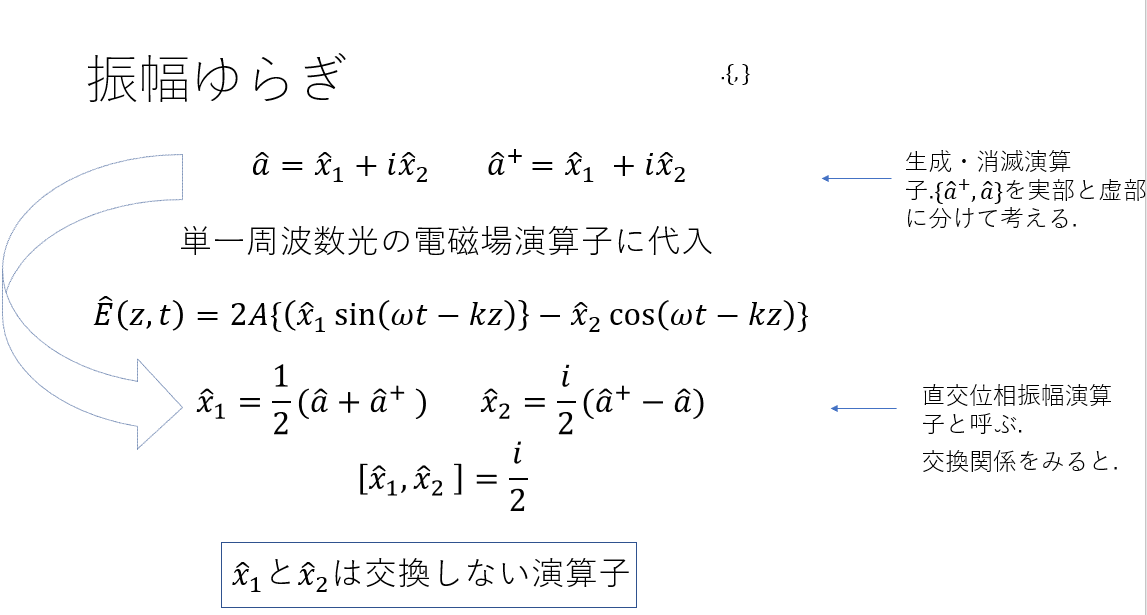
\includegraphics[width=1.0\textwidth]{img/zemi12.png}
        \caption[sample image (png)]{振幅ゆらぎ.}
        \label{Fig:1_5_4}
    \end{figure}

    \figref{Fig:1_5_4}は複素振幅の実部と虚部を表す演算子($\hat{x_1}$),($\hat{x_2}$)の交換関係について説明している。

\begin{figure}[htbp]
        \centering   
        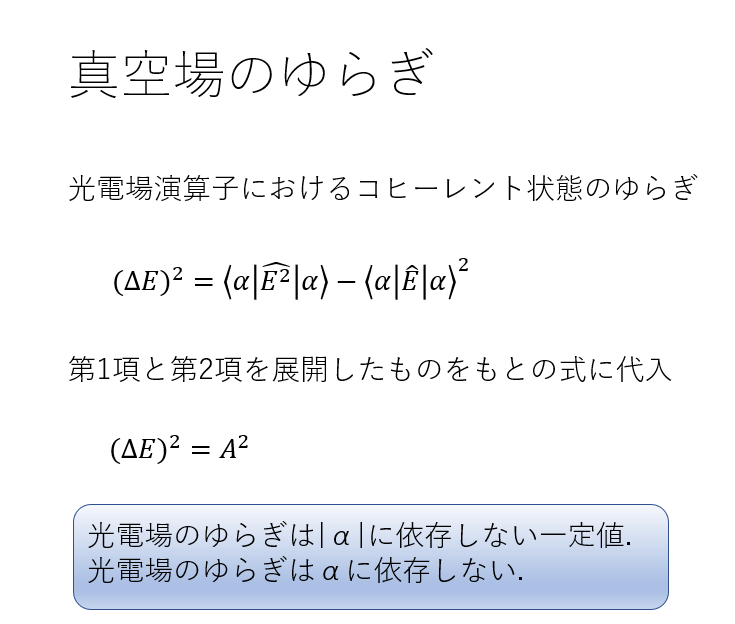
\includegraphics[width=0.8\textwidth]{img/zemi13.png}
        \caption[sample image (png)]{真空場のゆらぎ.}
        \label{Fig:1_5_5}
    \end{figure}
    \figref{Fig:1_5_5}は真空場のゆらぎについて説明しているこのゆらぎは$α$に依存しない.
    
\begin{figure}[htbp]
        \centering   
        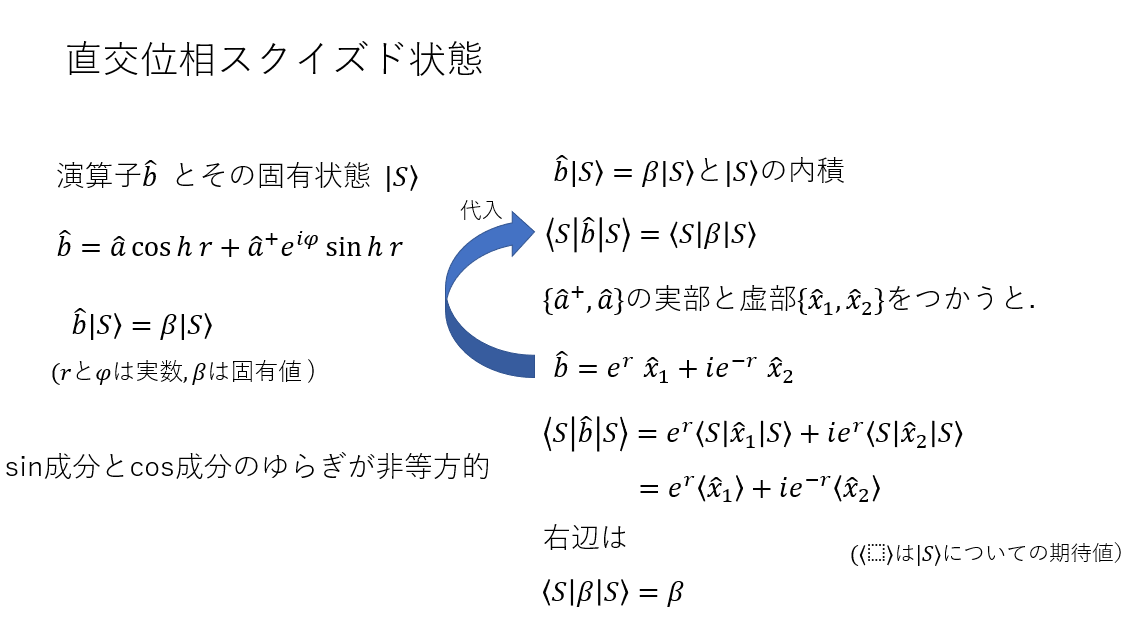
\includegraphics[width=1.0\textwidth]{img/zemi14.png}
        \caption[sample image (png)]{直交スクイズド状態.}
        \label{Fig:1_5_6}
    \end{figure}
    \figref{Fig:1_5_6}はスクイズド状態について説明している。直交位相スクイズド状態は演算子($\hat{b}$)とその固有状態$|{S}\rangle$として与えられる。

